\documentclass{article}
\usepackage{amsmath}
\usepackage{tikz}
\usetikzlibrary{arrows.meta}

\begin{document}

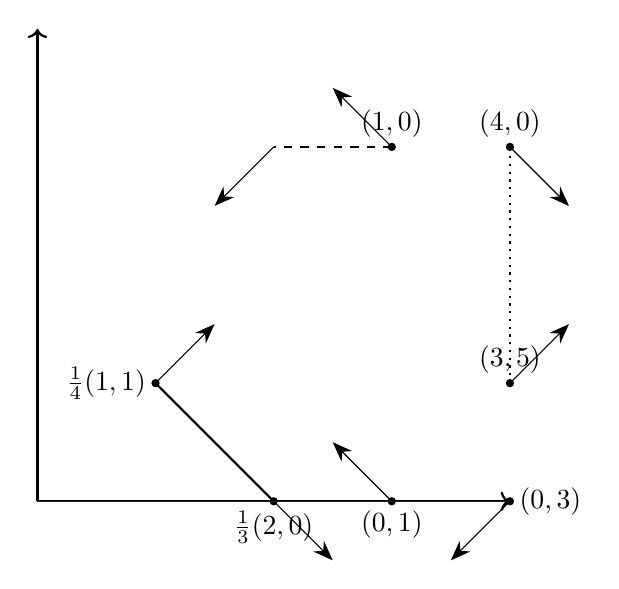
\begin{tikzpicture}[scale=1.5]
    % Define coordinates
    \coordinate (A) at (0,0);
    \coordinate (B) at (4,0);
    \coordinate (C) at (0,4);
    \coordinate (D) at (3,5);
    \coordinate (E) at (1,1);
    \coordinate (F) at (2,0);
    \coordinate (G) at (3,0);
    \coordinate (H) at (4,0);
    \coordinate (I) at (4,1);
    \coordinate (J) at (4,3);
    \coordinate (K) at (3,3);
    \coordinate (L) at (2,3);

    % Draw lines
    \draw[->, thick] (A) -- (B);
    \draw[->, thick] (A) -- (C);
    \draw[thick] (E) -- (F);
    \draw[dotted, thick] (G) -- (H);
    \draw[dotted, thick] (I) -- (J);
    \draw[dashed, thick] (K) -- (L);

    % Draw points
    \fill (E) circle (1pt) node[left] {$\frac{1}{4}(1,1)$};
    \fill (F) circle (1pt) node[below] {$\frac{1}{3}(2,0)$};
    \fill (G) circle (1pt) node[below] {$(0,1)$};
    \fill (H) circle (1pt) node[right] {$(0,3)$};
    \fill (I) circle (1pt) node[above] {$(3,5)$};
    \fill (J) circle (1pt) node[above] {$(4,0)$};
    \fill (K) circle (1pt) node[above] {$(1,0)$};

    % Draw arrows
    \draw[-{Stealth[scale=1.5]}] (E) -- ++(0.5,0.5);
    \draw[-{Stealth[scale=1.5]}] (F) -- ++(0.5,-0.5);
    \draw[-{Stealth[scale=1.5]}] (G) -- ++(-0.5,0.5);
    \draw[-{Stealth[scale=1.5]}] (H) -- ++(-0.5,-0.5);
    \draw[-{Stealth[scale=1.5]}] (I) -- ++(0.5,0.5);
    \draw[-{Stealth[scale=1.5]}] (J) -- ++(0.5,-0.5);
    \draw[-{Stealth[scale=1.5]}] (K) -- ++(-0.5,0.5);
    \draw[-{Stealth[scale=1.5]}] (L) -- ++(-0.5,-0.5);

    % Fill background
    \fill[gray!20] (A) -- (B) -- (H) -- cycle;
\end{tikzpicture}

\end{document}